\chapter{Progettazione concettuale}
\section{Analisi dei dati}
Le entità che possono essere individuate nel problema sono elencate all'interno della Tabella \ref{tab:entities}.
\begin{table}[h!]
\begin{tabularx}{\textwidth}{|l|X|}
\hline
\textbf{Entità} & \textbf{Descrizione} \\
\hline
\textbf{Conferenza} & Per le conferenze delle quali si vuole poter gestire le informazioni. Di ogni conferenza si conservano il \textit{nome}, la \textit{data di inizio} e di \textit{fine} e una \textit{descrizione}. \\ \hline
\textbf{Ente} & Per gli enti che organizzano le conferenze scientifiche. Di ogni ente si conserva solo il \textit{nome}. \\ \hline
\textbf{Sponsor} & Per gli sponsor che coprono le spese della conferenza. Di ogni sponsor si conserve solo il \textit{nome}.\\ \hline
\textbf{Comitato} & Per i gruppi di organizzatori che si occupano della gestione della conferenza scientifica. Si distinguono in comitati \textit{scientifici} e \textit{locali}. \\ \hline
\textbf{Organizzatore} & Per i membri dei comitati scientifici e locali. Di ogni organizzatore si riportano \textit{titolo, nome, cognome, email} ed \textit{istituzione di afferenza}. \\ \hline
\textbf{Sede} & Per descrivere il luogo dove si tengono le varie conferenze. Di ogni sede si conservano: \textit{nome, indirizzo, città} e il \textit{codice di indirizzamento postale}. \\ \hline
\textbf{Sala} & Per tenere traccia dell'ubicazione delle varie sessioni. Di ogni sala si conserva il \textit{nome della sala} e la sua \textit{capacità}. \\ \hline
\textbf{Sessione} & Per rappresentare le sessioni di una conferenza. Per ogni sessione si riporta il \textit{titolo} e le date di \textit{inizio} e di \textit{fine}. \\ \hline
\textbf{Programma} & Per il programma di ciascuna sessione. Ogni programma contiene la specifica del \textit{coordinatore} della sessione ed eventualmente la presenza di un \textit{keynote speaker}, ovvero un partecipante di rilievo. \\ \hline
\textbf{Intervento} & Per i vari interventi di una sessione. Per ogni intervento si conserva un \textit{abstract}, il partecipante (\textit{speaker}) che effettua l'intervento e l'\textit{orario} dello stesso. \\ \hline
\textbf{Partecipante} & Per i partecipanti delle varie sessioni. Ogni partecipante ha gli stessi attributi degli organizzatori. \\ \hline
\textbf{Intervallo} & Per descrivere i vari intervalli presenti all'interno di una sessione. Questi possono essere di tue tipologie: coffee break oppure dei pranzi. Per ogni intervallo si riporta l'\textit{orario}. \\ \hline
\textbf{Evento sociale} & Per i vari eventi sociali previsti all'interno di una sessione. Questi possono essere di varia natura. Come per gli intervalli se ne riporta l'\textit{orario}. \\ \hline
\textbf{Utente} & Per l'utente di un applicativo che interagisce con la base di dati. Di ogni utente si conservano gli stessi dati di un organizzatore. In aggiunta è presente un attributo per la \textit{password}. \\
\hline
\end{tabularx}
\caption{Entità del problema}\label{tab:entities}
\end{table}
\newpage
\section{Schema concettuale}
\begin{figure}[h!]
\centering
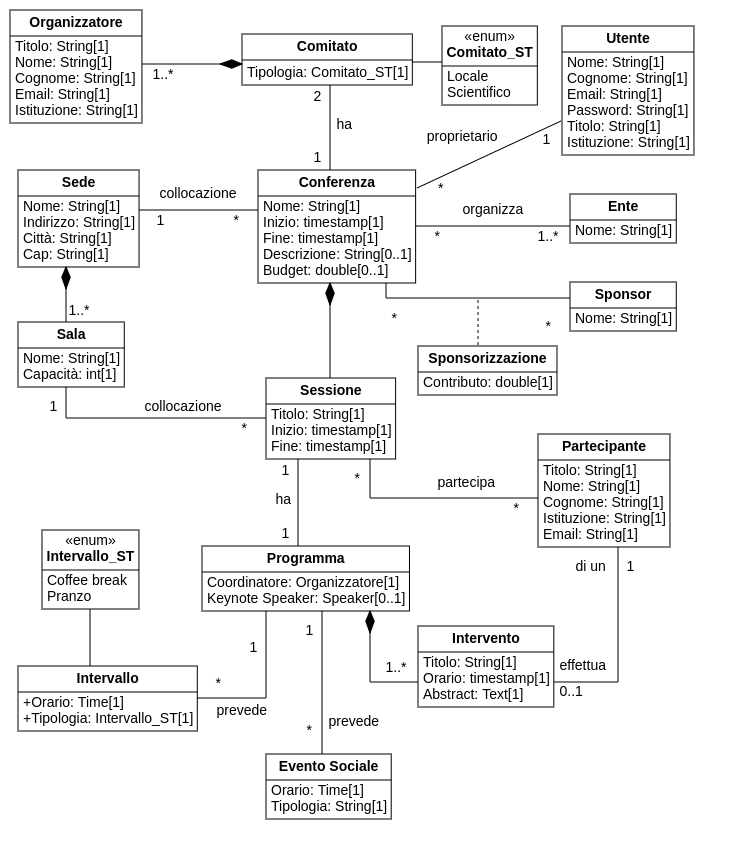
\includegraphics[scale=0.6]{Immagini/Schema_Concettuale.png}
\caption{Schema concettuale del problema}\label{uml:schema_concettuale}
\end{figure}
Nella Figura \ref{uml:schema_concettuale} è presente lo schema concettuale della base di dati descritta nella sezione \ref{sez:traccia}.
\section{Ristrutturazione dello schema concettuale}

